\documentclass[10pt,a4paper]{article}
\usepackage[utf8]{inputenc}
\usepackage[italian]{babel}
\usepackage{amsmath}
\usepackage{amsfonts}
\usepackage{amssymb}
%aggiungi pacchetto che commenti
\usepackage{comment}
\usepackage{graphicx}
\usepackage[left=2cm,right=2cm,top=2cm,bottom=2cm]{geometry}
\newcommand{\rem}[1]{[\emph{#1}]}
\newcommand{\exn}{\phantom{xxx}}

\author{Gruppo 23 \\ Alessandro Costanzo Ciano, Luca Palumbo}
\title{N.D02: Latch, contatori e shift-register}
\begin{document}
\date{16 aprile 2024}
\maketitle

\section{D-Latch con Enable}
\subsection{Montaggio}
Il circuito è stato montato come da schema, utilizzando le porte NAND come indicato in figura. Gli ingressi DATA (D) ed ENABLE (E) sono stati collegati ad altrettanti pattern di tipo “Clock” dell’AD2 sincroni (cioè di frequenza di circa 1 kHz) e sfasati di 90 gradi.

\begin{figure}[htp]
\begin{center}
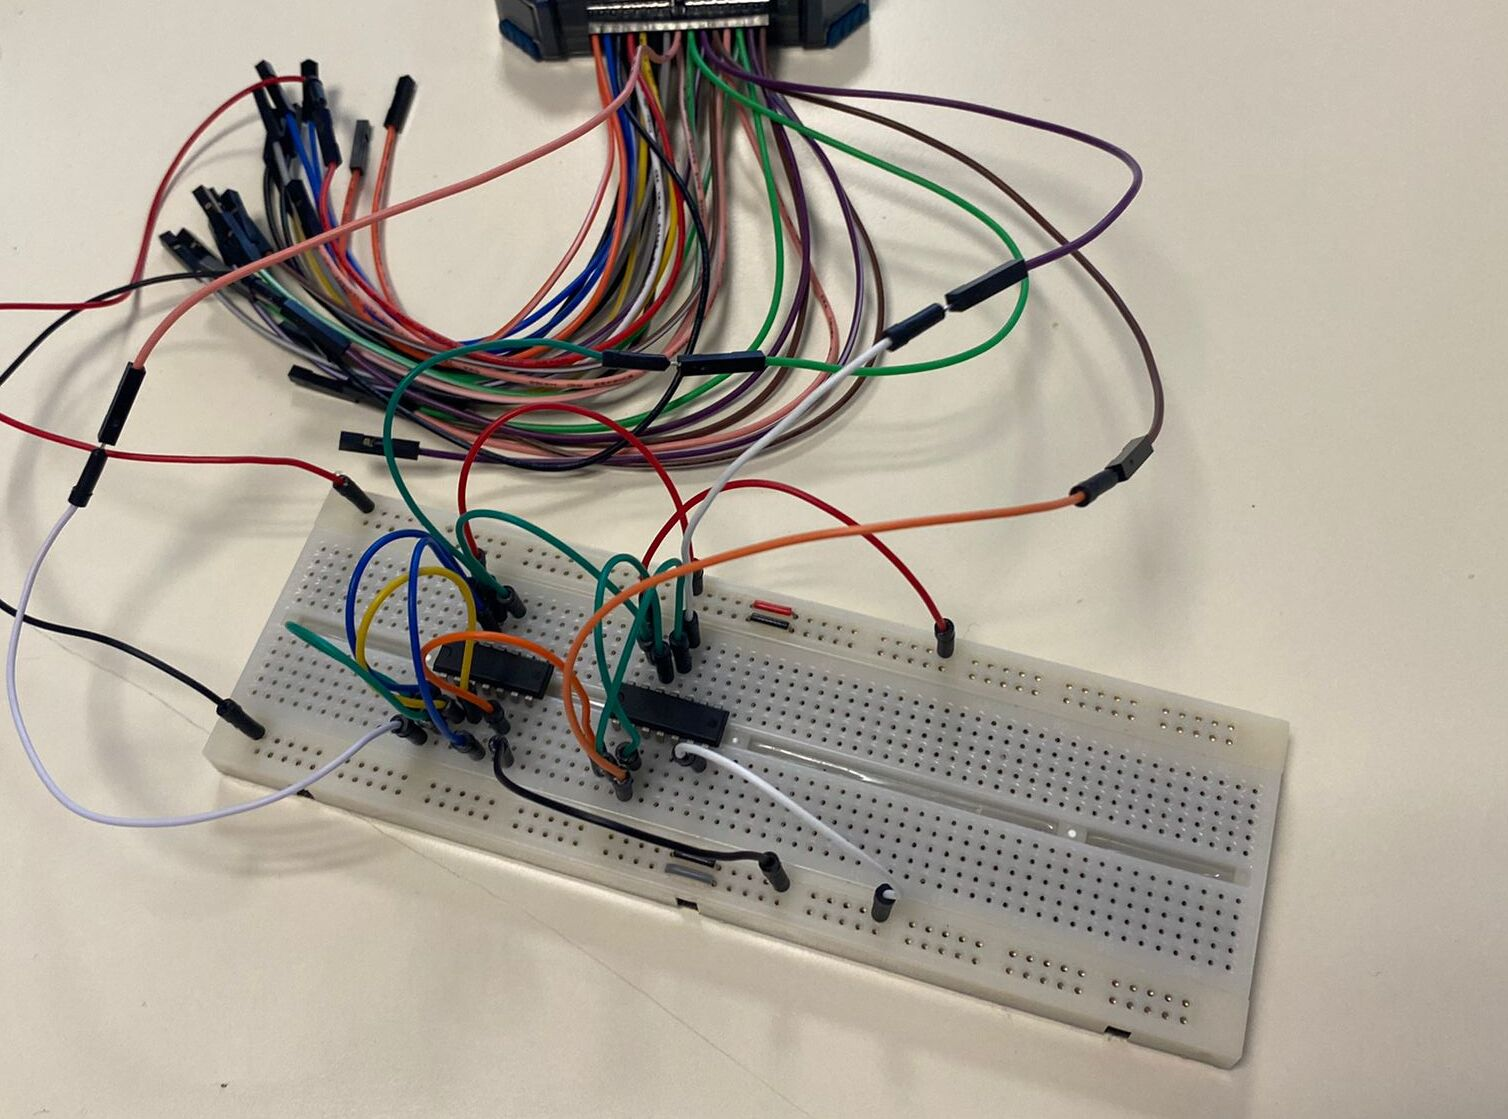
\includegraphics[scale=0.25]{circuito1.jpeg}
\caption{Foto del circuito D-Latch con enable.}
\end{center}
\end{figure}

\subsection{Funzionamento}
Il circuito è un D-Latch con enable. Il ruolo degli ingressi D ed E è il seguente: l'ingresso D è l'ingresso di dati, mentre l'ingresso E è l'ingresso di abilitazione. Se E è alto, il latch è abilitato e il valore in D viene trasmesso in uscita. Se E è basso, il latch è disabilitato e il valore in uscita rimane invariato. 
\subsection{Verifica}
Il funzionamento del Latch è stato verificato osservando l’andamento dei segnali D, EN e Q (inviati ad altrettante linee di Logic), confrontando la successione osservata degli stati con quanto previsto dalla tabella delle verità (per E = 0 Q rimane costante e immune a variazioni di D, viceversa per E = 1). Gli screen-shot relativi sono riportati in figura \ref{fig1}.

\begin{figure}[htp]
\begin{center}
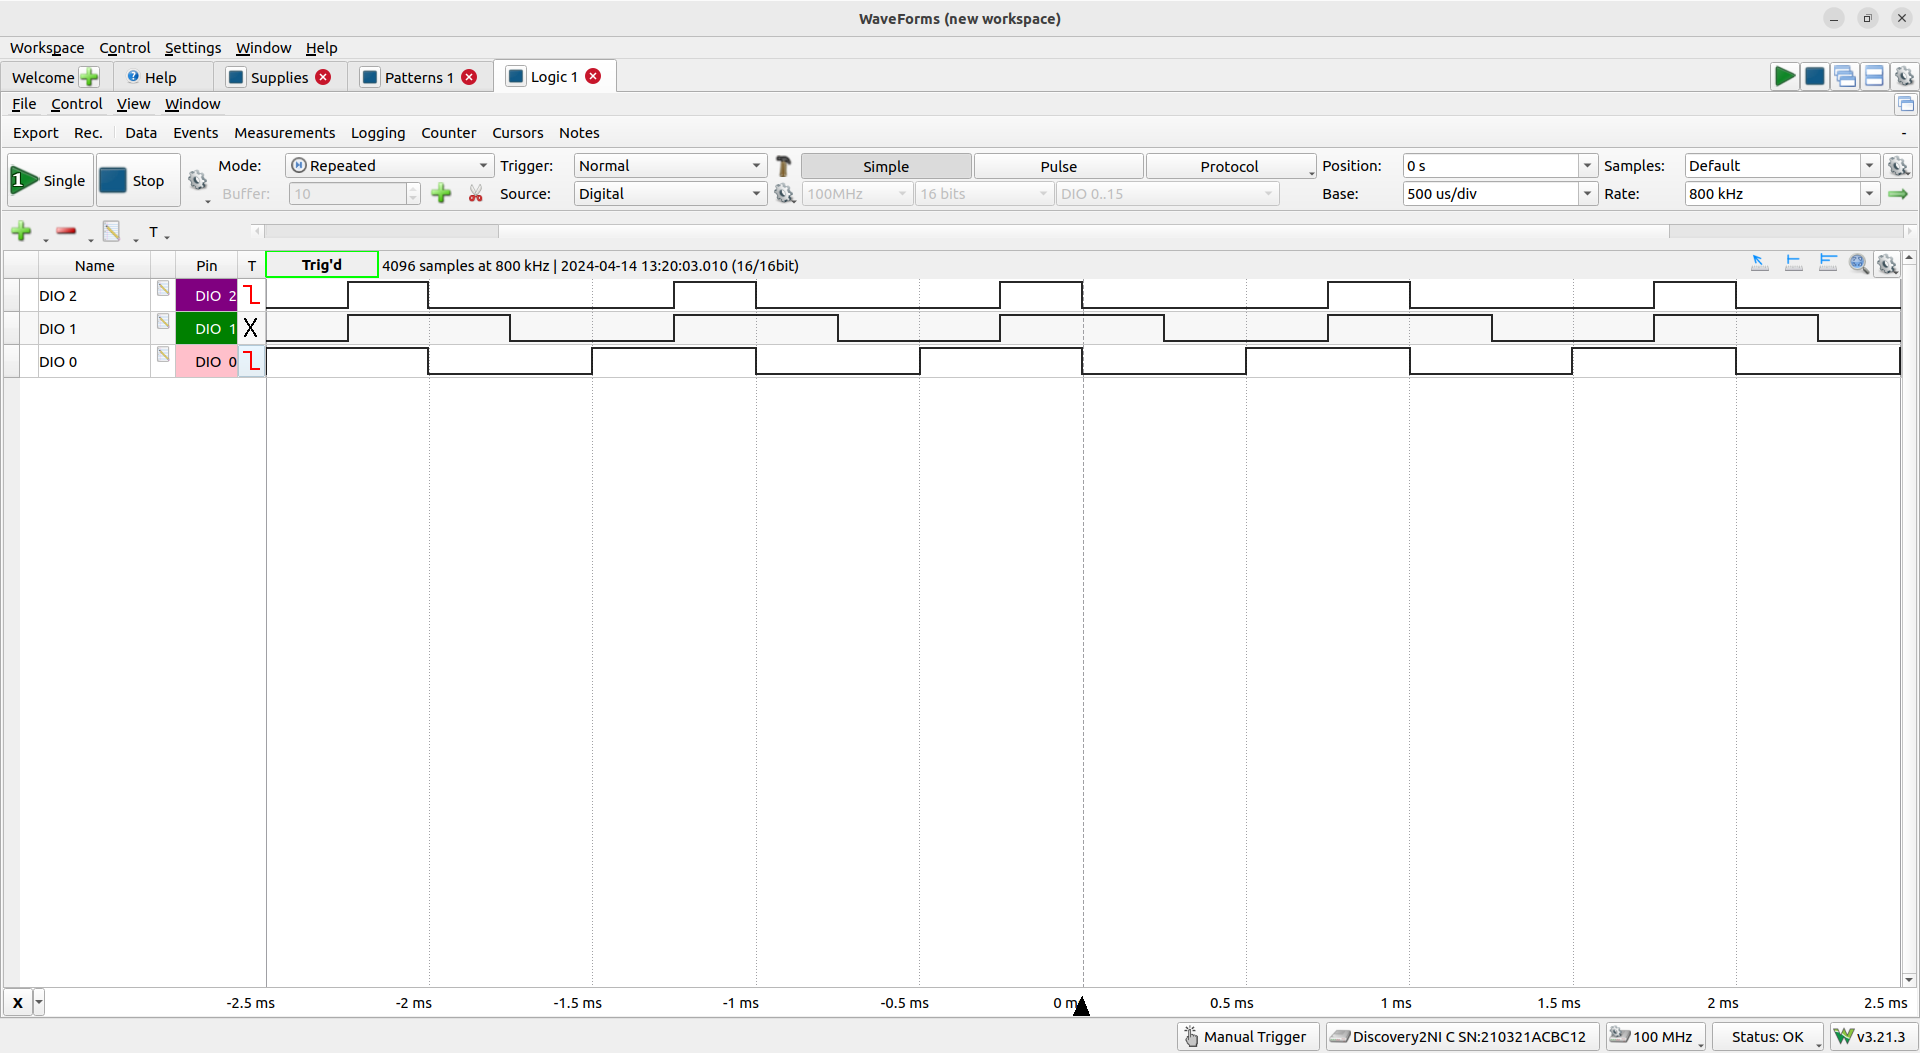
\includegraphics[scale=0.25]{fig1.png}
\caption{Screen-shot relativi al funzionamento del D-Latch con enable. DIO 0 = D, DIO 1 = E , DIO 2 = Q.}
\label{fig1}
\end{center}
\end{figure}

\section{Shift register con edge-triggered D-Flip Flop}
\subsection{Montaggio}
Il circuito è stato montato come da schema, utilizzando 2 integrati 74LS74 (ciascuno con due FF di tipo D) seguendo lo schema in figura. Gli ingressi di preset di tutti i FF sono stati collegati ad uno StaticIO di tipo “Button” e polarità tale che l’uscita sia 1=released, 0=pressed. L’ingresso D del FF0 è stato collegato ad uno staticIO di tipo Switch in modalità Push-Pull. Il Clock è stato pilotato con un segnale di tipo Clock di Pattern. Ogni uscita dei FF è stata collegata a canali dello StaticIO di tipo LED-software.

\begin{figure}[htp]
\begin{center}
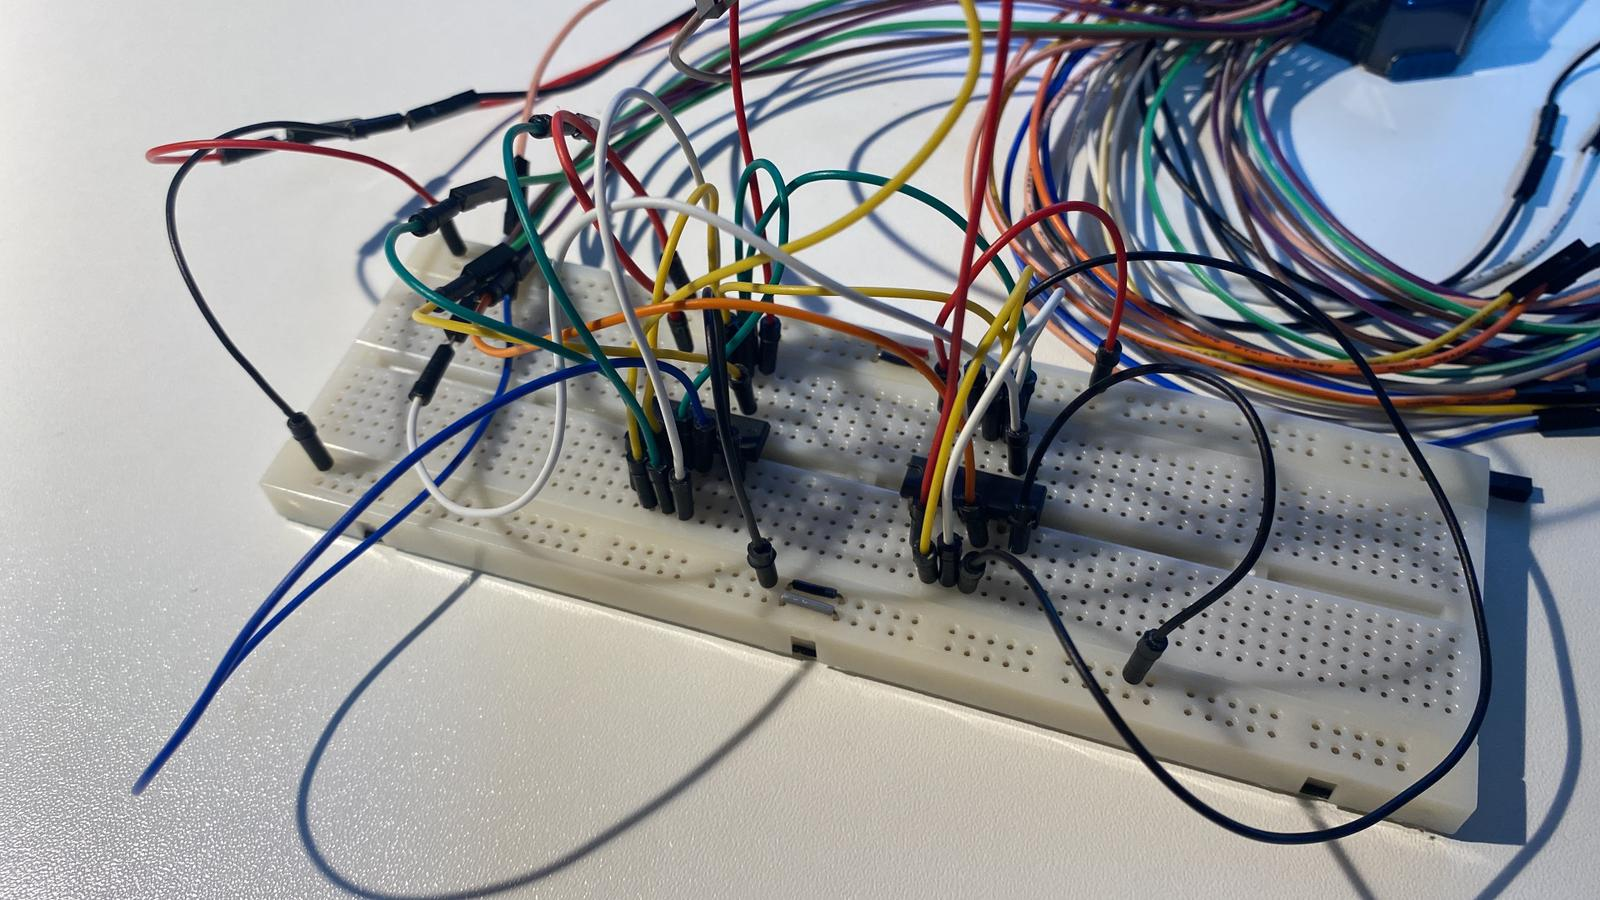
\includegraphics[scale=0.25]{circuito2.jpeg}
\caption{Prima foto del circuito shift register.}
\end{center}
\end{figure}

\begin{figure}[htp]
    \begin{center}
    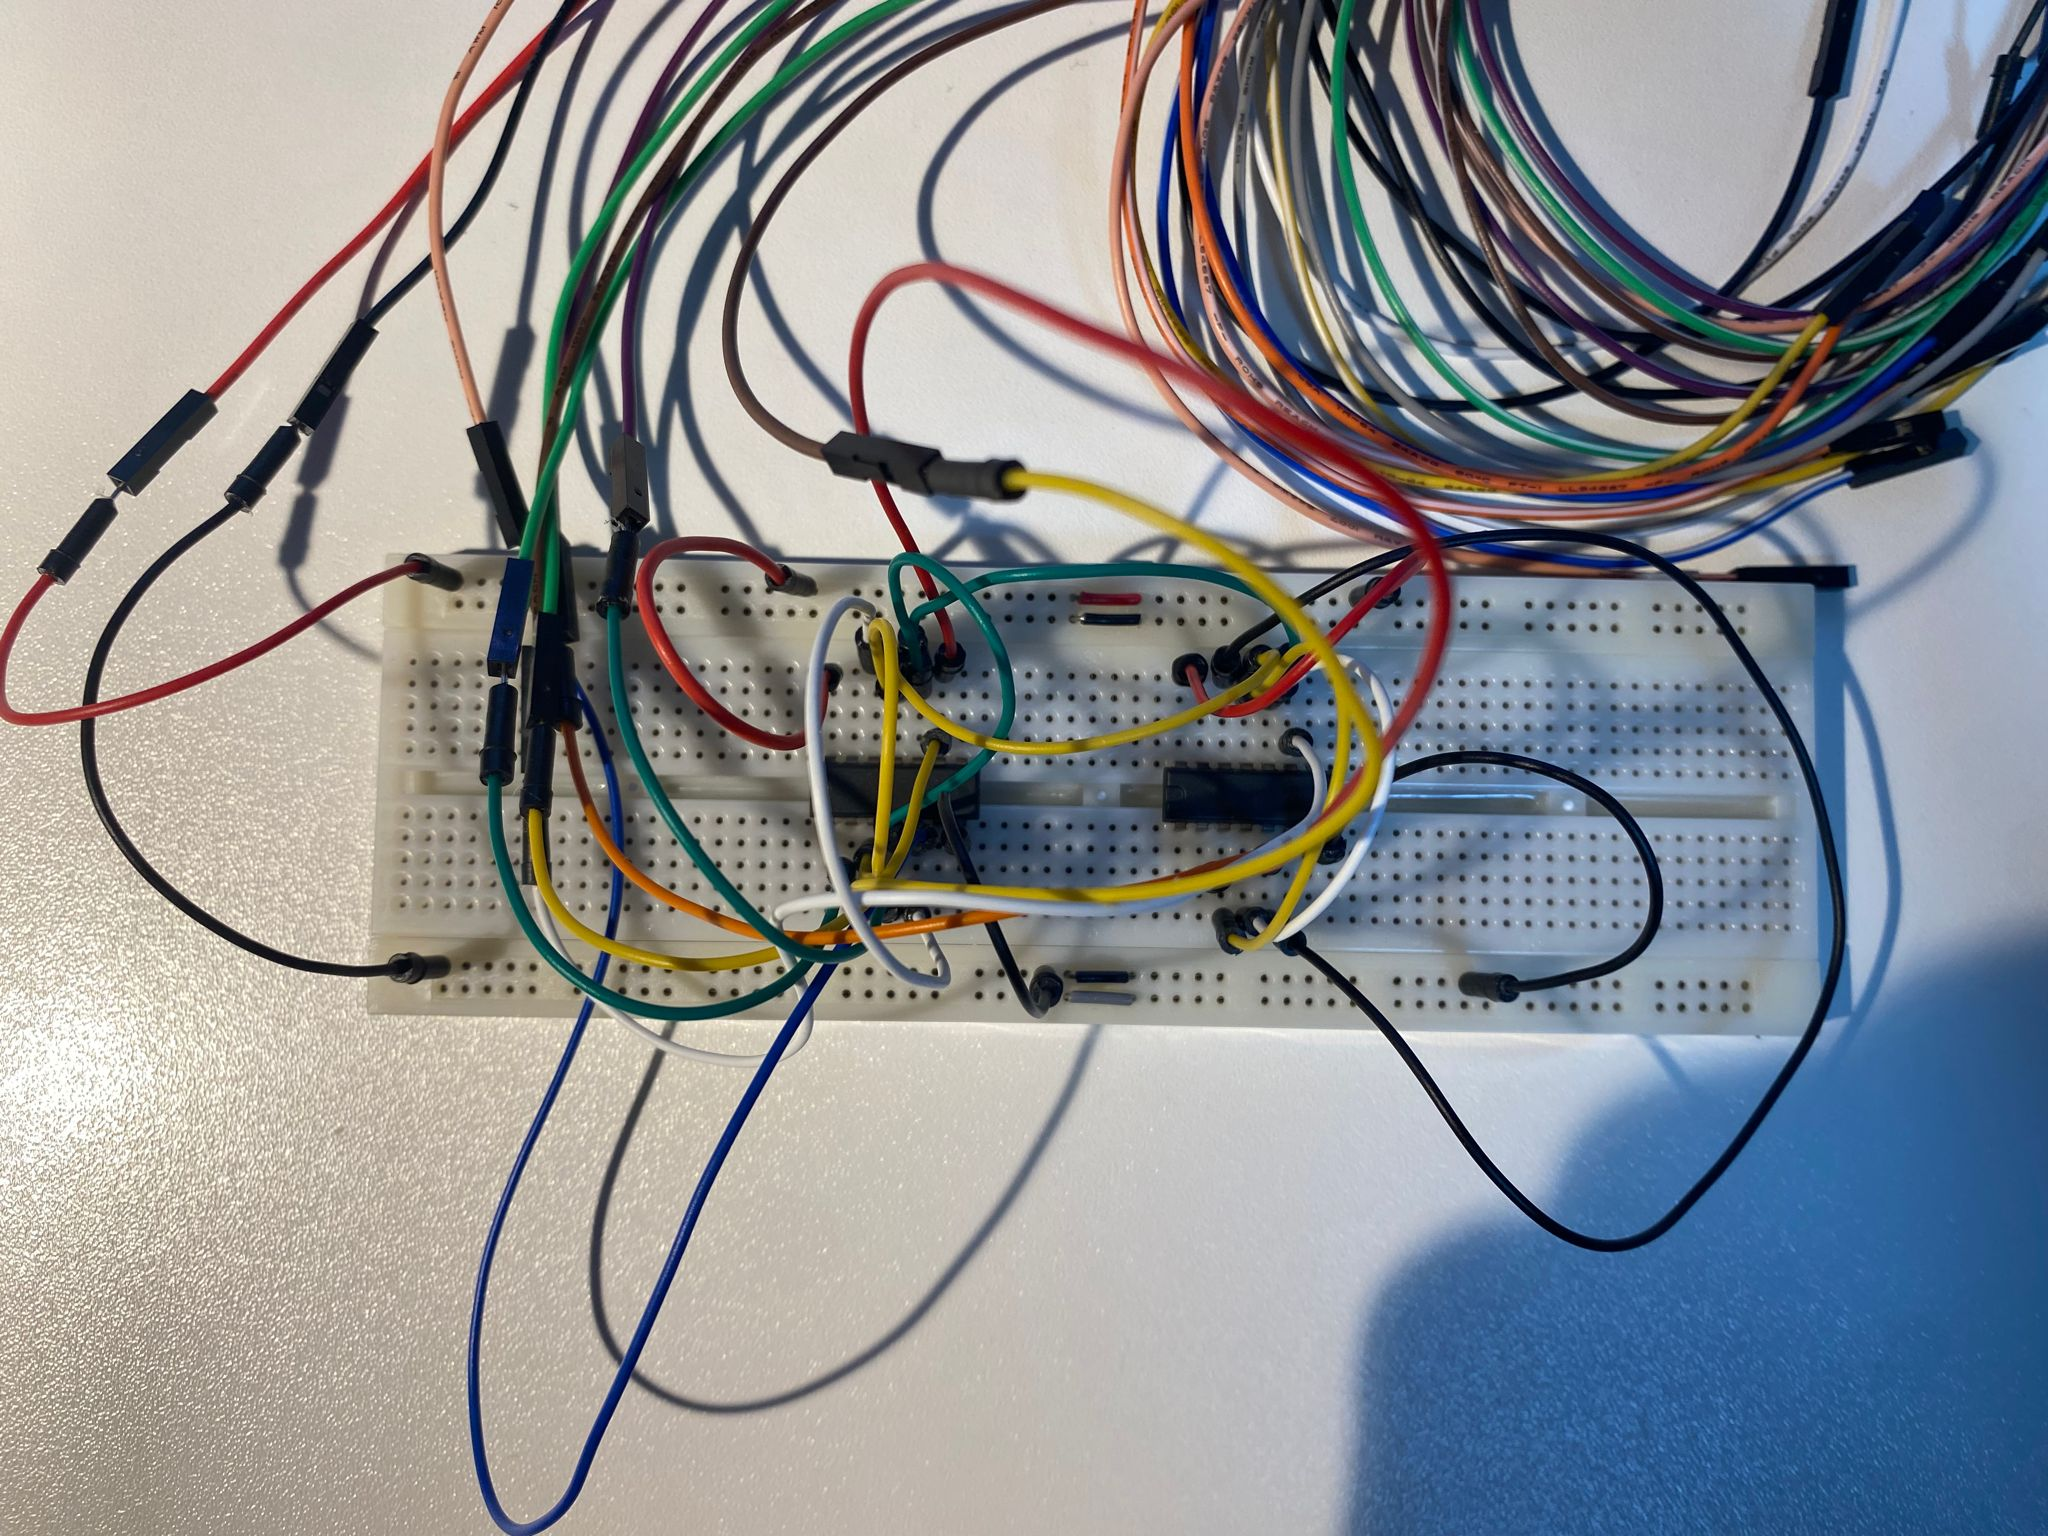
\includegraphics[scale=0.18]{circuitodoppio.jpeg}
    \caption{Seconda foto del circuito shift register.}
    \end{center}
    \end{figure}

\subsection{Funzionamento e verifica}
Il circuito è uno shift register a 4 bit. Il pulsante collegato al preset porta lo shift register nello stato 1111. La commutazione delle uscite è asincrona, ossia avviene indipendentemente dal Clock.
Disabilitato il preset, è stato inviato un Clock di bassa frequenza (~1 Hz). Il funzionamento del circuito è stato verificato controllando l’accensione/spegnimento dei LED-software in corrispondenza a successive commutazioni del D-switch: lasciando i preset alti le uscite cambiano progressivamente stato (a partire da $Q_0$, verso $Q_3$) ad ogni fronte di salita del Clock in base all'ingresso B. 
Usando sia il D-switch che il preset, è stato verificato che l'ingresso che guida le uscite è il preset (agendo indipendentemente dal Clock).
Collegando l’uscita NOT(Q3) all’ingresso D del primo FF (al posto del Switch) e utilizzando un clock ad alta frequenza (~1 kHz), sui piedini di uscita Q[3..0] si osservano le forme d'onda in figura \ref{fig2}. Il funzionamento del circuito è il seguente: il clock ad alta frequenza fa sì che tutte uscite cambino stato ad ogni fronte di salita, trasmettendo il valore di NOT(Q3) al primo FF, che lo trasmette al secondo FF e così via, ottenendo uno shift register: partendo da una configurazione 1111 è chiaro che si passerà a 0111 e 0011 negli stati successivi, e così via fino ad arrivare a 0000, da cui si riparte ciclicamente.
\begin{figure}[htp]
\begin{center}
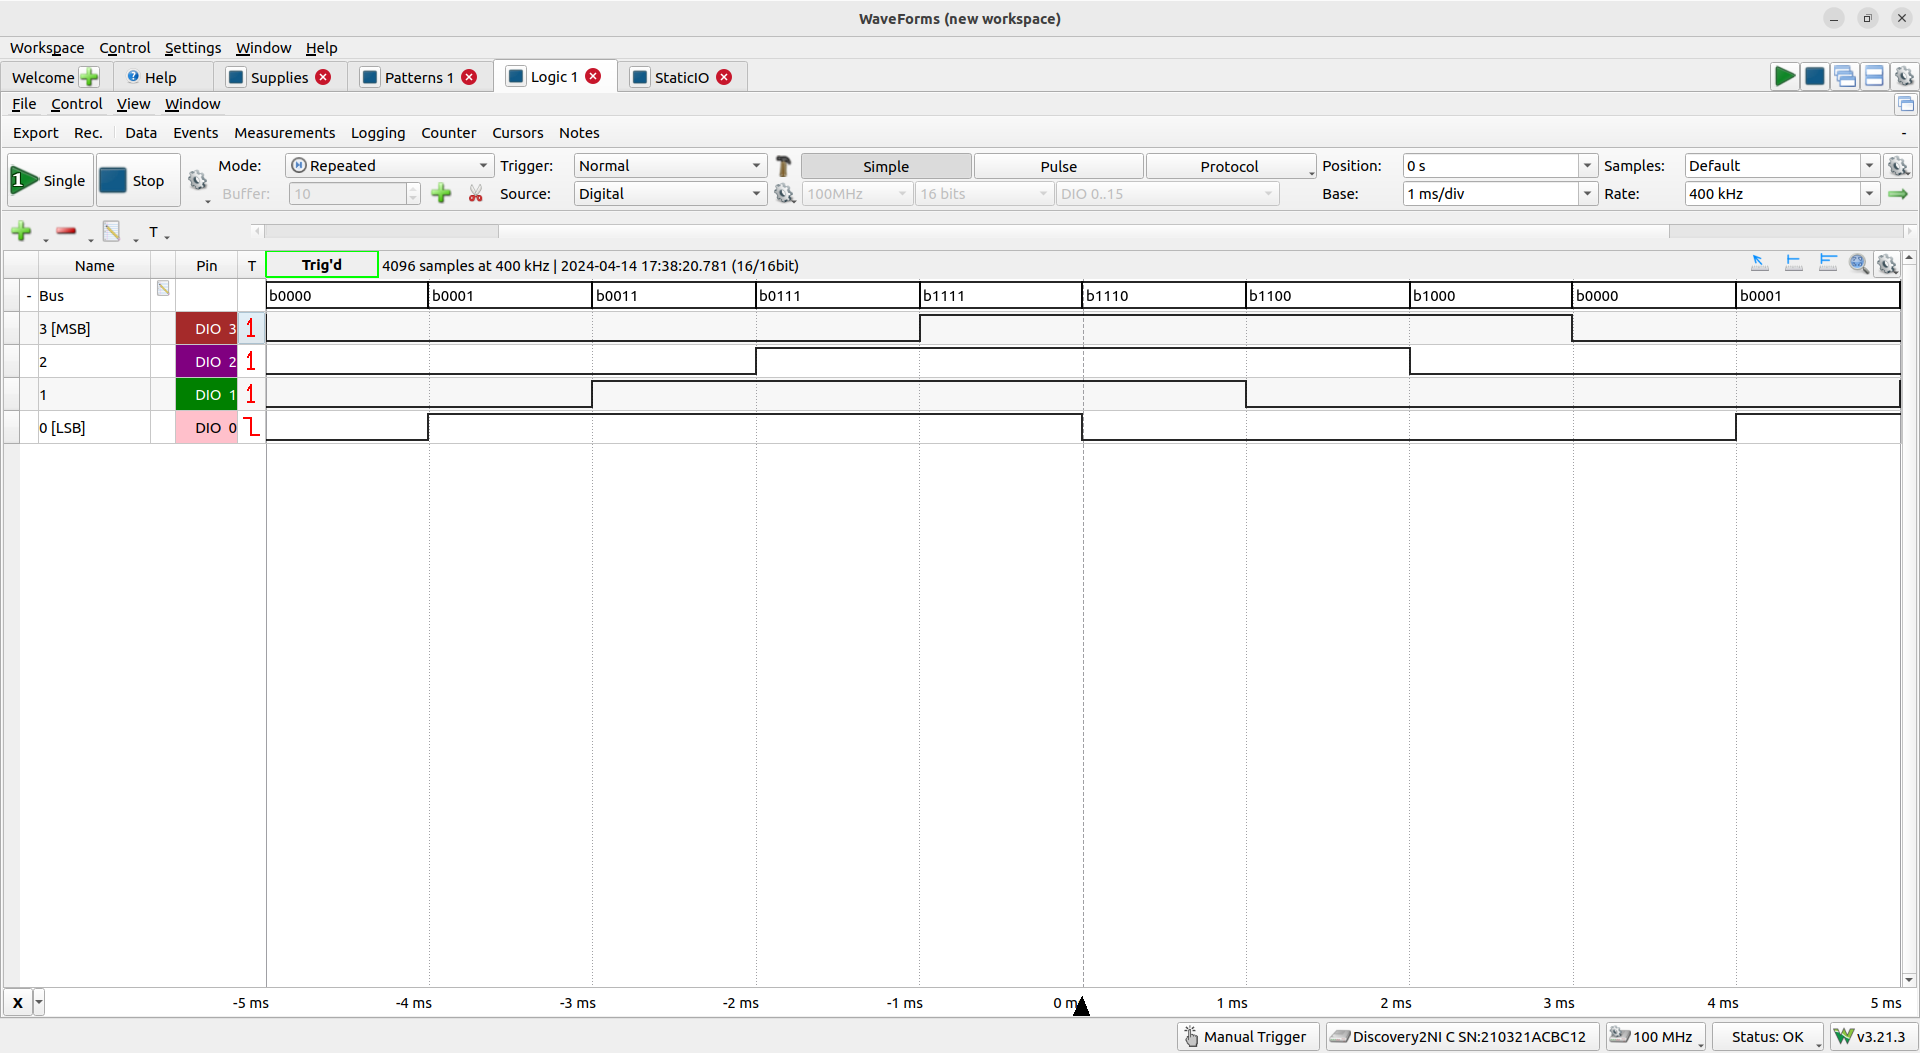
\includegraphics[scale=0.25]{fig2.png}
\caption{Forme d'onda osservate sui piedini di uscita Q[3..0] del circuito shift register.}
\label{fig2}
\end{center}
\end{figure}

\section{Utilizzo di un contatore come divisore di frequenza}
\subsection{Montaggio}
Il circuito è stato montato come da schema, utilizzando il contatore a 4 bit sincrono 74LS163. Le 4 uscite sono state collegate ad un bus con altrettanti bit di Logic. Il clock è stato inviato ad una frequenza di circa 10 kHz. 

\begin{figure}[htp]
\begin{center}
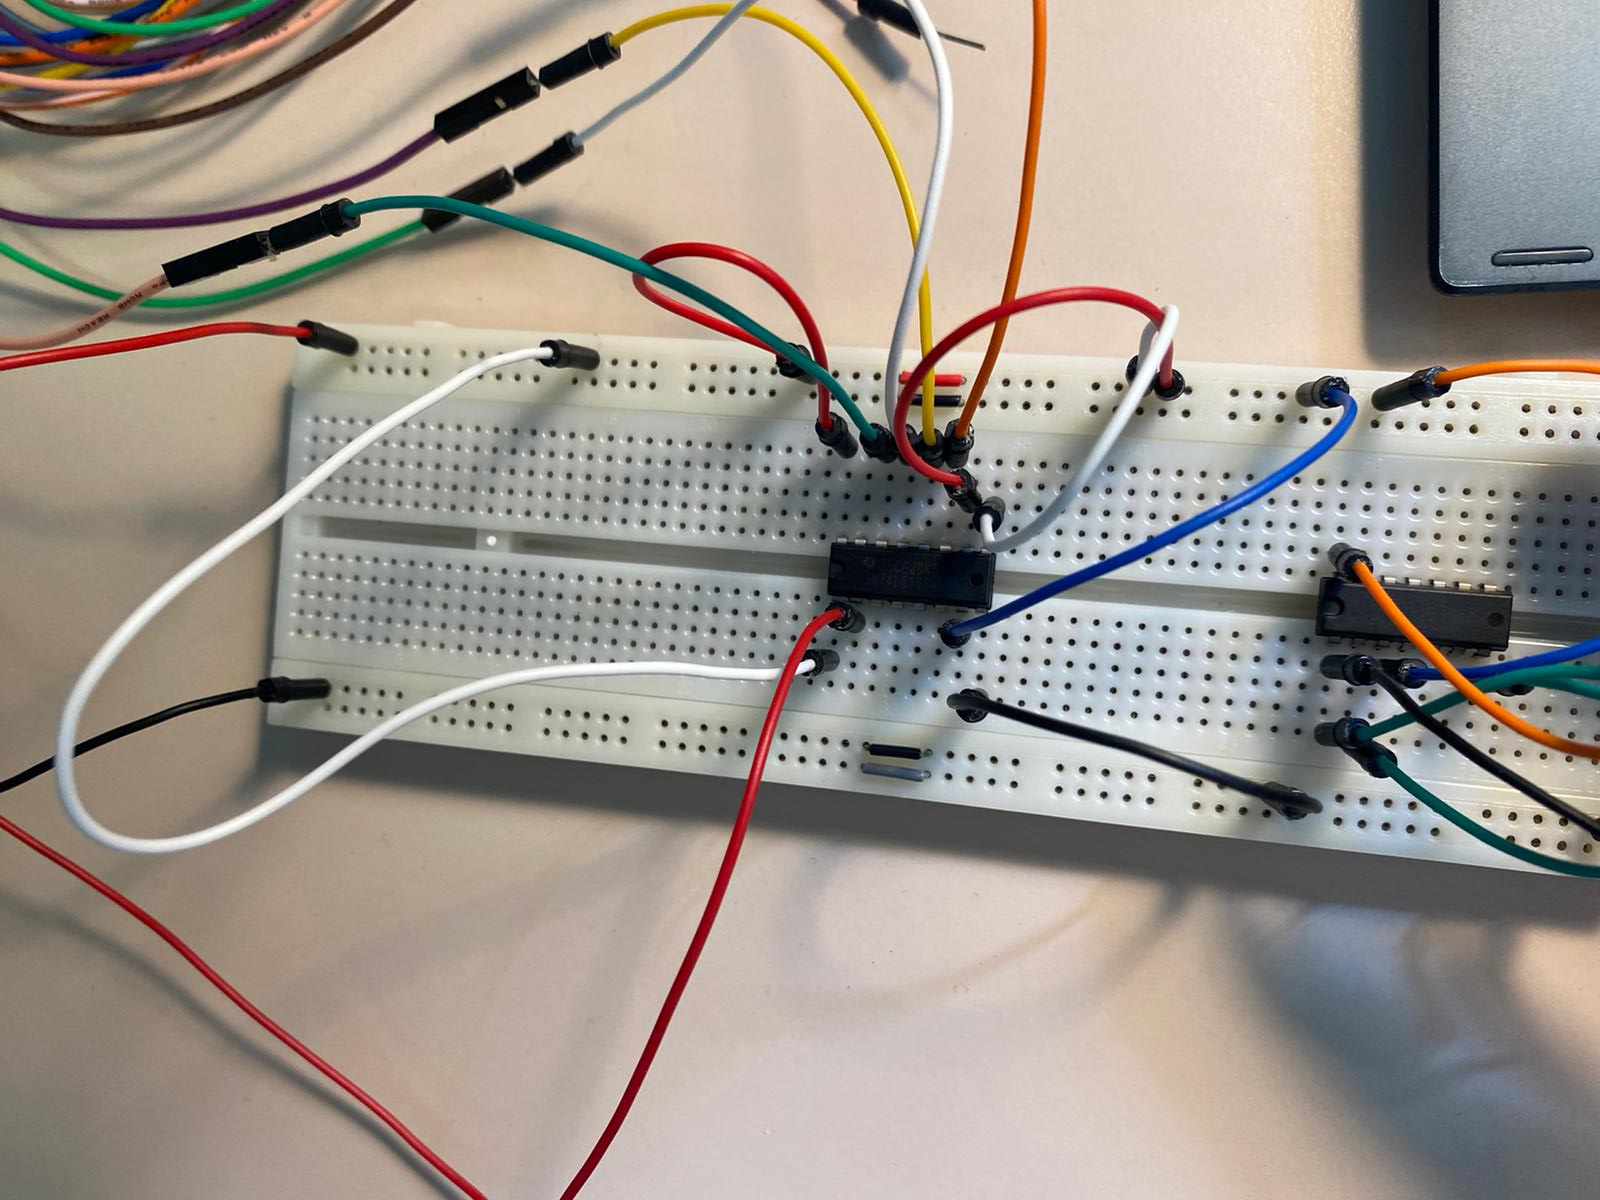
\includegraphics[scale=0.25]{circuito3.jpeg}
\caption{Foto del circuito contatore.}
\end{center}
\end{figure}

\subsection{Funzionamento e verifica}
Il circuito agisce come contatore: visualizzando il valore del bus si osserva che il contatore conta da 0 a 15 e riparte ciclicamente. Osservando individualmente i segnali Q0, Q1, Q2 e Q3 si verifica che la loro frequenza risulti pari rispettivamente ad 1/2, 1/4, 1/8, 1/16 della frequenza di clock. Il comportamento sincrono del contatore è stato verificato in figura \ref{fig3}. 
Per verificare il comportamento sincrono del contatore, si è visualizzato contemporaneamente il fronte del clock e quello dei singoli bit di uscita alla transizione del contatore 15→0. Riducendo la larghezza della scala temporale fino a poche decine di ns, si osserva che i bit di uscita cambiano stato in modo sincrono al fronte di discesa del clock (figura \ref{fig4}).

\begin{figure}[htp]
\begin{center}
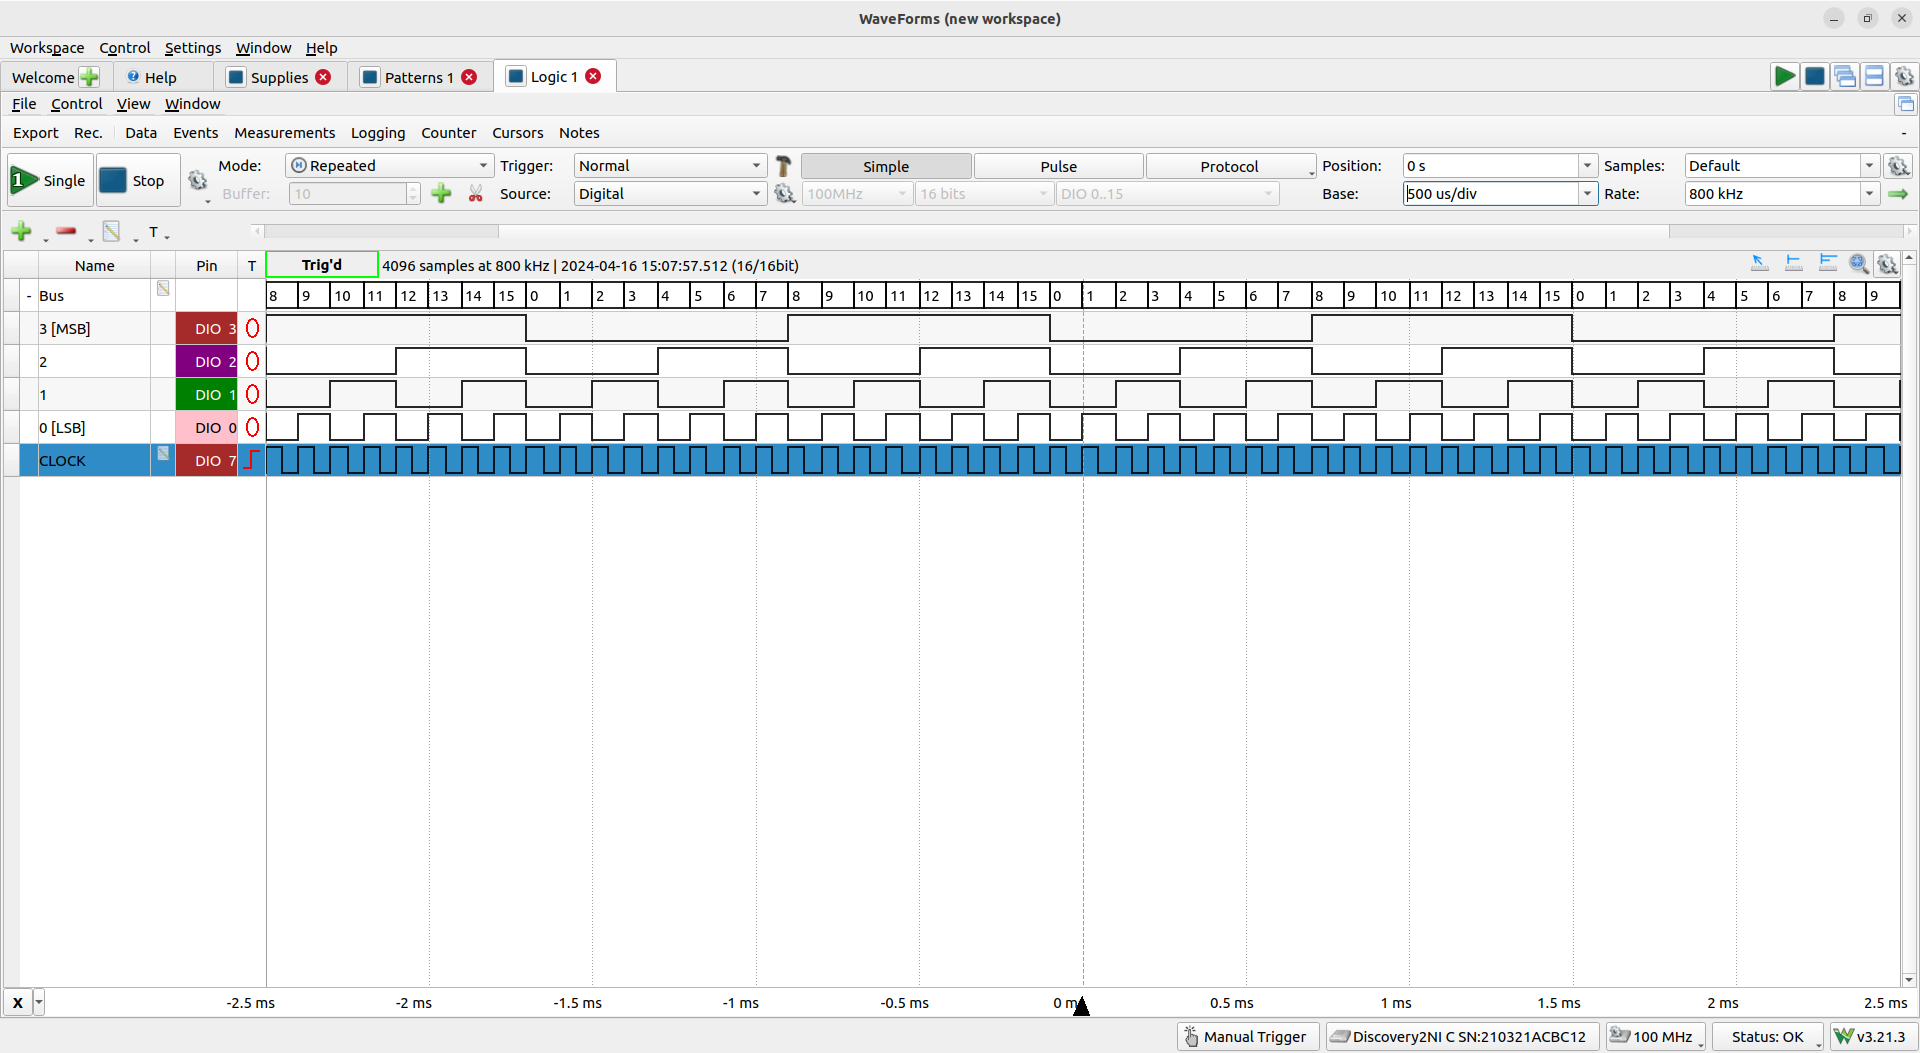
\includegraphics[scale=0.25]{fig3.png}
\caption{Comportamento sincrono del contatore.}
\label{fig3}
\end{center}
\end{figure}

\begin{figure}[htp]
\begin{center}
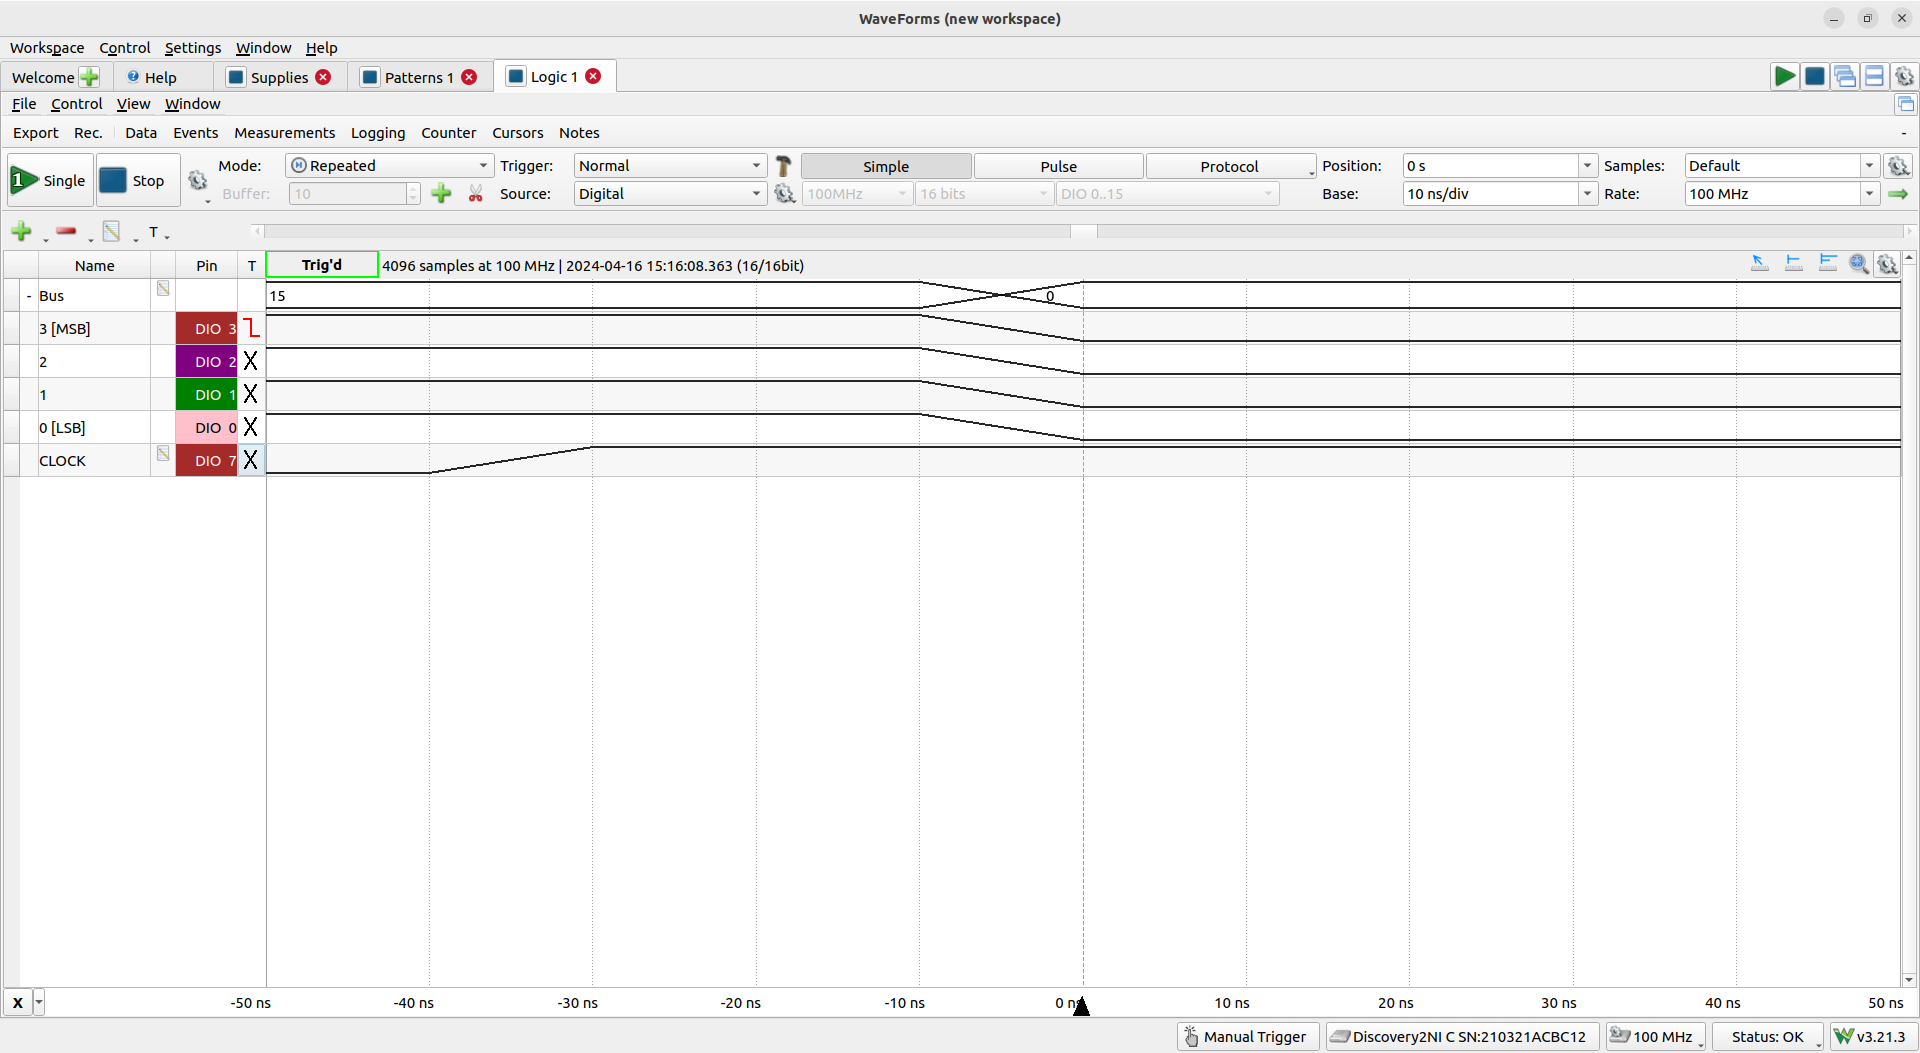
\includegraphics[scale=0.25]{fig4.png}
\caption{Comportamento sincrono del contatore a scala temporale ridotta.}
\label{fig4}
\end{center}
\end{figure}

\subsection{Divisore di frequenza 1/10}
Per costruire un divisore di frequenza 1/10 si è progettato un circuito che conta 10 stati, in modo da avere un segnale di frequenza 1/10 della frequenza di clock utilizzando il load sincrono. Il circuito è stato montato come da schema, utilizzando l'RCO per generare il segnale di Load. Il valore iniziale del contatore è stato caricato mediante Pattern (bus a 4 bit di tipo costante) collegando i canali DIO 8-11 alle linee di ingresso del contatore (figura \ref{fig5_1}). Il valore iniziale del contatore è stato scelto come 6. Il funzionamento del circuito è il seguente: il contatore conta da 6 a 15 e riparte ciclicamente, generando un segnale di Load che abilita il caricamento.

\begin{figure}[htp]
\begin{center}
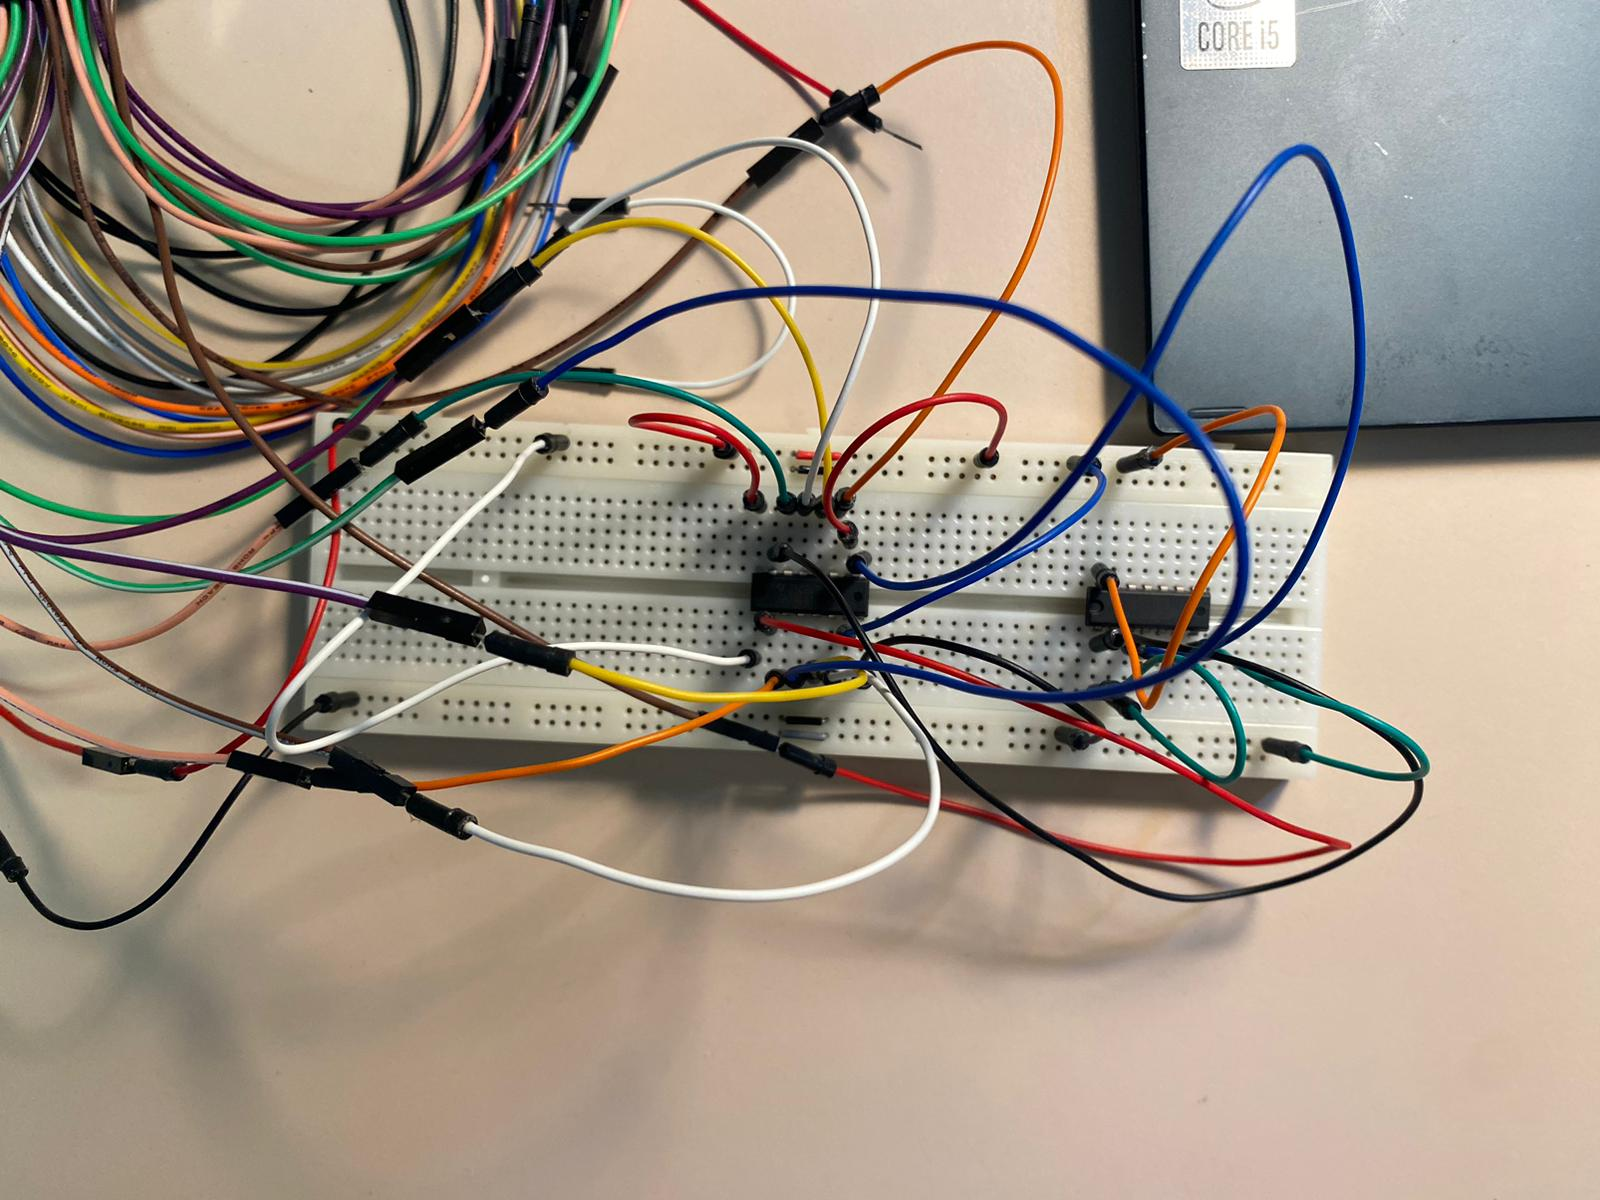
\includegraphics[scale=0.25]{circuito4.jpeg}
\caption{Foto del circuito divisore di frequenza 1/10.}
\end{center}
\end{figure}

\begin{figure}[htp]
\begin{center}
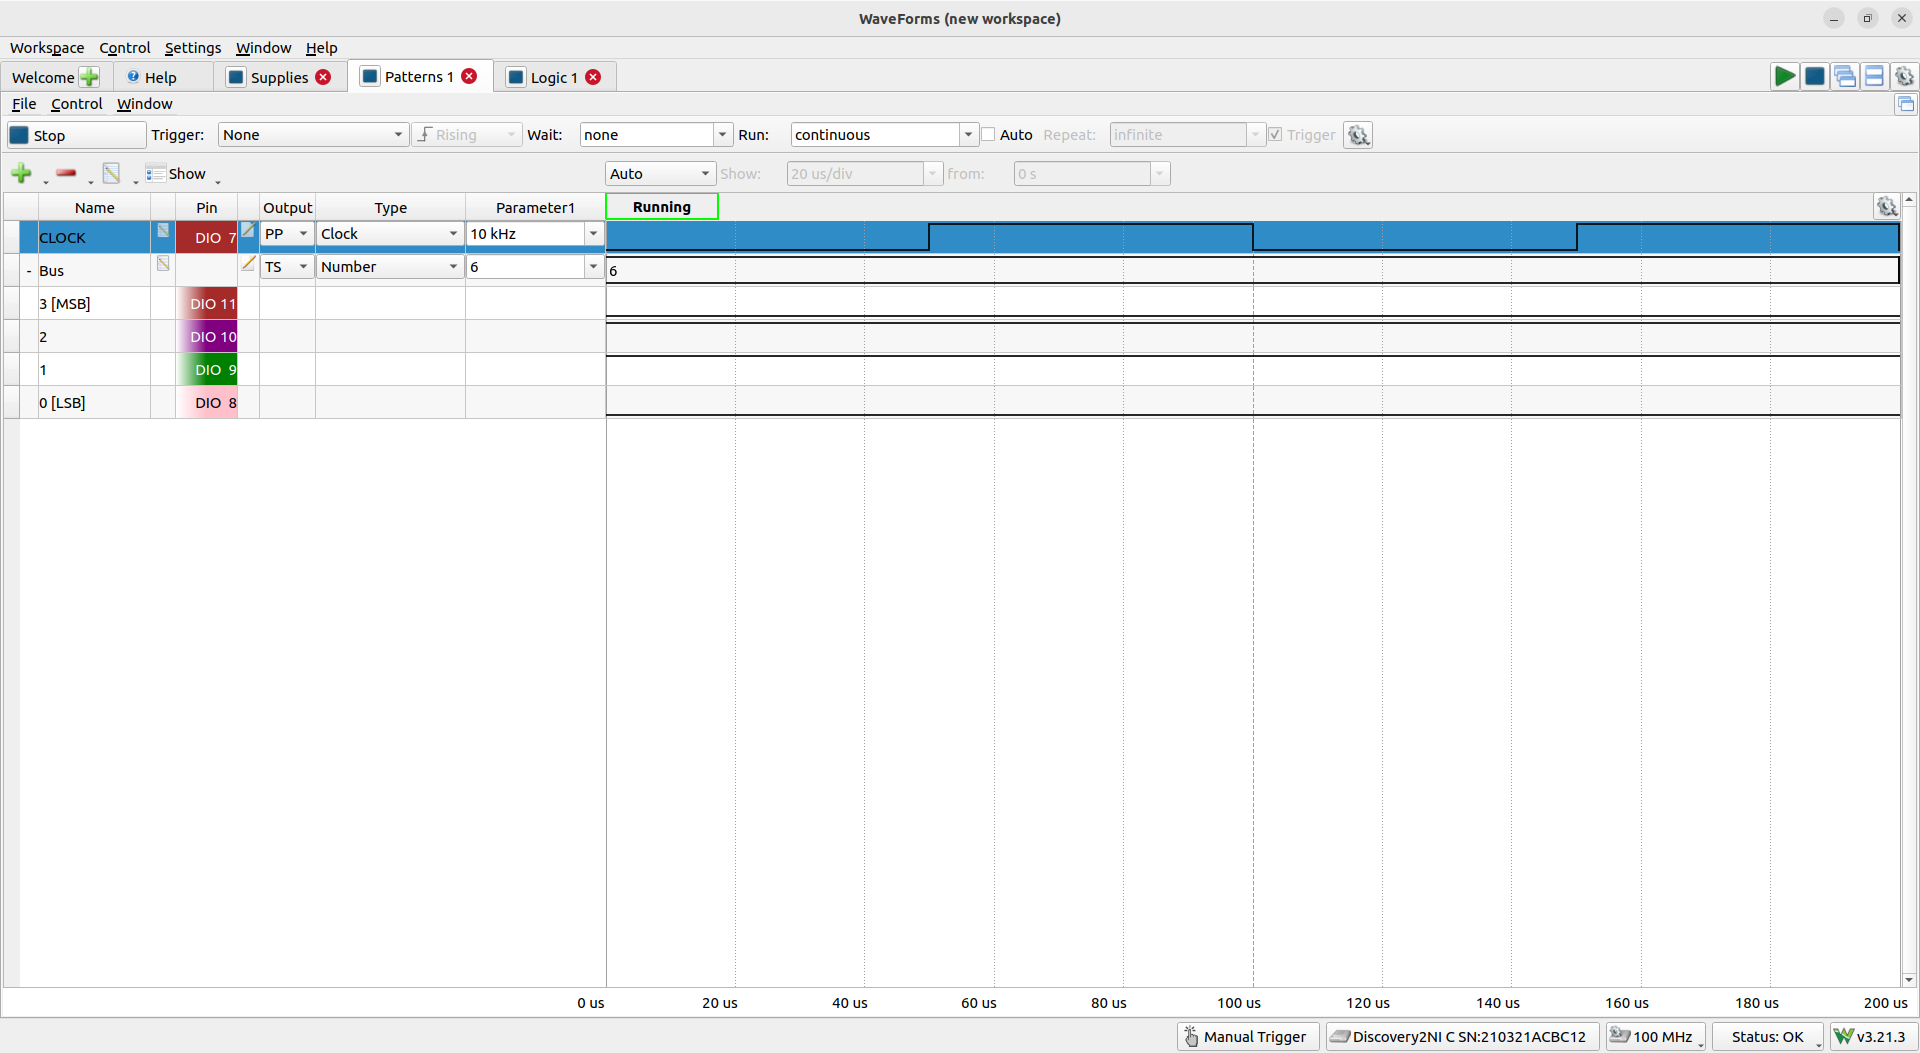
\includegraphics[scale=0.25]{fig5_1.png}
\caption{Valori iniziali di ingresso e Clock.}
\label{fig5_1}
\end{center}
\end{figure}

\begin{figure}[htp]
\begin{center}
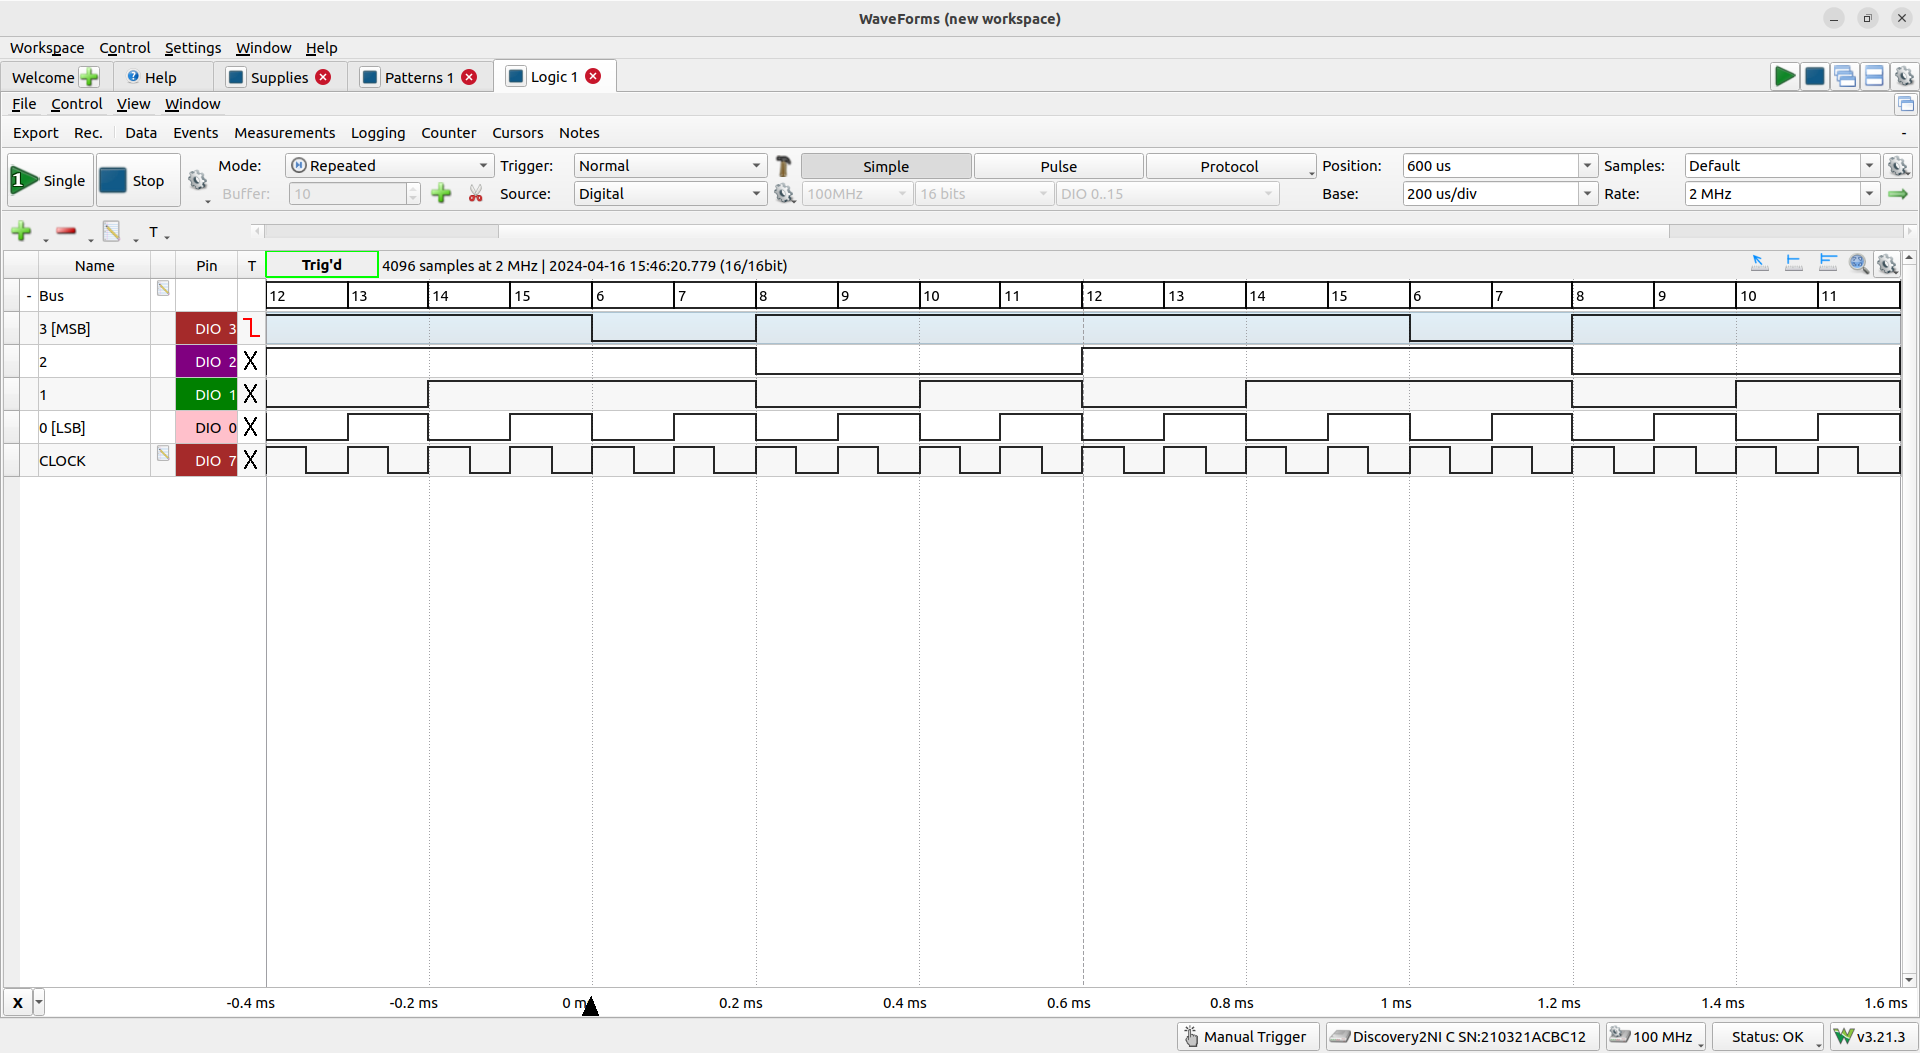
\includegraphics[scale=0.25]{fig5.png}
\caption{Comportamento del divisore di frequenza 1/10.}
\label{fig5}
\end{center}
\end{figure}

%da qui le indicazioni da seguire
\begin{comment}
Laboratorio di Fisica 3 BASE
Prof. Nicolò e Prof.ssa C.Roda
Esercitazione N. D2
Latch, contatori e shift-register
Questa esercitazione ha lo scopo di costruire alcuni circuiti logici sequenziali, progressivamente
più complessi. Si raccomanda di eseguire un montaggio ordinato e pianificare lo spazio sulla
basetta. Utilizzare fili di opportuna lunghezza e cercando di rispettare un codice colori
consistente (ad es. fili di colore rosso e nero per l’alimentazione e la massa, un unico colore per
la distribuzione del clock, etc.).
1) Materiale a disposizione. Consultare i data-sheet per le piedinature e le caratteristiche
degli integrati:
• SN74LS00 Quad NAND Gate
• SN74LS163 4-bit synchronous binary counter with synchronous clear/load
• SN74LS74 Dual D-Latch
• SN74LS86 Quad XOR Gate
2) D-Latch con Enable
a. Montare un D-Latch con enable utilizzando le
porte NAND come indicato in figura. Collegare
gli ingressi DATA (D) ed ENABLE (E) ad
altrettanti pattern di tipo “Clock” dell’AD2
sincroni (cioè di frequenza di circa 1 kHz) e
sfasati di 90 gradi.
b. Spiegare brevemente il funzionamento del
circuito indicando il ruolo degli ingressi D ed EN.
c. Verificare il funzionamento del Latch osservando l’andamento dei segnali D, EN e Q
(inviati ad altrettante linee di Logic), confrontando la successione osservata degli stati
con quanto previsto dalla tabella delle verità ed allegando gli screen-shot necessari.
3) Shift register con edge-triggered D-Flip Flop
a. Si costruisca uno shift register a 4 bit utilizzando 2
integrati 74LS74 (ciascuno con due FF di tipo D)
seguendo lo schema in figura. Collegare:
i. gli ingressi di preset di tutti i FF ad uno
StaticIO di tipo “Button” e polarità tale
che l’uscita sia 1=released, 0=pressed;
ii. l’ingresso D del FF0 ad uno staticIO di
tipo Switch in modalità Push-Pull.
iii. Pilotare il Clock con un segnale di tipo
clock di Pattern.
iv. Ogni uscita dei FF a canali dello
StaticIO di tipo LED-software.
b. Utilizzare il pulsante collegato al preset per portare
lo shift register nello stato 1111. La commutazione
delle uscite è sincrona o asincrona?
c. Disabilitato il preset, inviare un clock di bassa
frequenza (~1 Hz). Verificare controllando
l’accensione/spegnimento dei LED-software il funzionamento del circuito incorrispondenza a successive commutazioni del D-switch. Provare anche inizializzazioni
diverse da 1111.
d. Verificate quale ingresso guida le uscite se utilizzate sia il D-switch che il preset.
e. Si colleghi l’uscita NOT(Q3) all’ingresso D del primo FF (al posto del Switch).
Utilizzando un clock ad alta frequenza (~1 kHz) si descrivano le forme d’onde e le
frequenze osservate sui piedini di uscita Q[3..0] collegate ad un bus di Logic in ordine
di significatività. Spiegare il funzionamento del circuito.
NB: in teoria gli ingressi CLR (negato) e PRE (negato) possono essere lasciati disconnessi, ma
se si dovessero osservare malfunzionamenti, potrebbe essere opportuno collegarli ai 5V
attraverso una resistenza di pull-up da 1k.
4) Utilizzo di un contatore come divisore di frequenza
a. Si vuole costruire un divisore di frequenza binario (x2,
x4, x8, x16) utilizzando il contatore a 4 bit sincrono
74LS163. Montare il circuito come in figura,
collegando le 4 uscite ad un bus con altrettanti bit di
Logic, anche in questo caso rispettando l’ordine di
significatività.
b. Inviare un clock di frequenza circa 10 kHz e verificare
che il circuito agisca come contatore visualizzando il
valore del bus su una finestra temporale di durata pari
a 20 periodi del Clock. Per una corretta
visualizzazione dell’intero ciclo del contatore,
potrebbe risultare conveniente impostare in Logic un
trigger di tipo “Protocol” con la richiesta bus=0.
c. Osservare individualmente i segnali Q0, Q1, Q2 e Q3
e verificare che la loro frequenza risulti pari rispettivamente ad 1/2, 1/4, 1/8, 1/16 della
frequenza di clock.
d. Verificare il comportamento sincrono del contatore visualizzando contemporaneamente
il fronte del clock e quello dei singoli bit di uscita alla transizione del contatore 15→0.
Impostare il trigger come al punto precedente e ridurre la larghezza della scala temporale
fino a poche decine di ns.
e. Progettare e costruire un circuito che conti 10 stati, in modo da avere segnale di frequenza
1/10 della frequenza di clock utilizzando il load sincrono. Montare il circuito e discuterne
il funzionamento indicando quale segnale abbia frequenza 1/10 della frequenza di clock
e con quale duty-cycle.
Suggerimento:
• utilizzare il “Ripple carry output” (RCO) per generale il segnale di “Load”
(prestare attenzione al fatto che il Load del 74LS163 è “active low” ed occorre
negare l’RCO prima di inviarlo).
• Caricare un valore iniziale nel contatore a seconda della divisione di frequenza
che si vuole ottenere. Il valore iniziale si può definire mediante Pattern (bus a 4
bit di tipo PP costante) oppure StaticIO (4 switch oppure lo slider) collegando
adeguatamente i canali DIO alle linee di ingresso D[3..0] del contatore (anche in
questo caso prestare attenzione all’ordine dei bit).
Verificare la corrispondenza tra fattore di divisione in frequenza del RCO rispetto al
Clock e valore iniziale del contatore e discutere il funzionamento del circuito.
\end{comment}

\end{document}


